\chapter{Obtención de los datos}

La siguiente figura (ENUMERAR FIGURAS) resume el proceso para la obtención de los datos. (REFERENCIA A REPO Y DISTINTOS SCRIPTS)

Los \textit{clips} utilizados para el entrenamiento del modelo son movimientos extraídos de videos de youtube. Para su obtención:

\begin{itemize}

\item Partiendo de un script que hace llamadas a \textit{yt-dlp} se descargan los videos correspondientes, con una resolución de 480p, y formato mp4, utilizando su url. (PONER URLS)

\item Los videos se introducen en \textit{supervisely} (SUPERVISELY ANEXO) para el etiquetado.

\begin{itemize}
\item Se han seleccionado 20 atletas (10 hombres y 10 mujeres), para los cuales de cada video se seleccionan 15 movimientos. De cada movimiento queda una muestra aproximadamente de 300 clips (video corto del movimiento).

\end{itemize}

\item Supervisely permite extraer un fichero json con las anotaciones generadas. Ejecutando el script \textit{manifester.py} generamos el fichero input que necesita el siguiente script.

\item Utilizando \textit{ffmpeg-split.py} se pasan las anotaciones generadas y los videos de referencia, y se obtienen los clips que se utilizarán posteriormente para entrenar el modelo.

\end{itemize}



\begin{figure}[H]
    \centering
		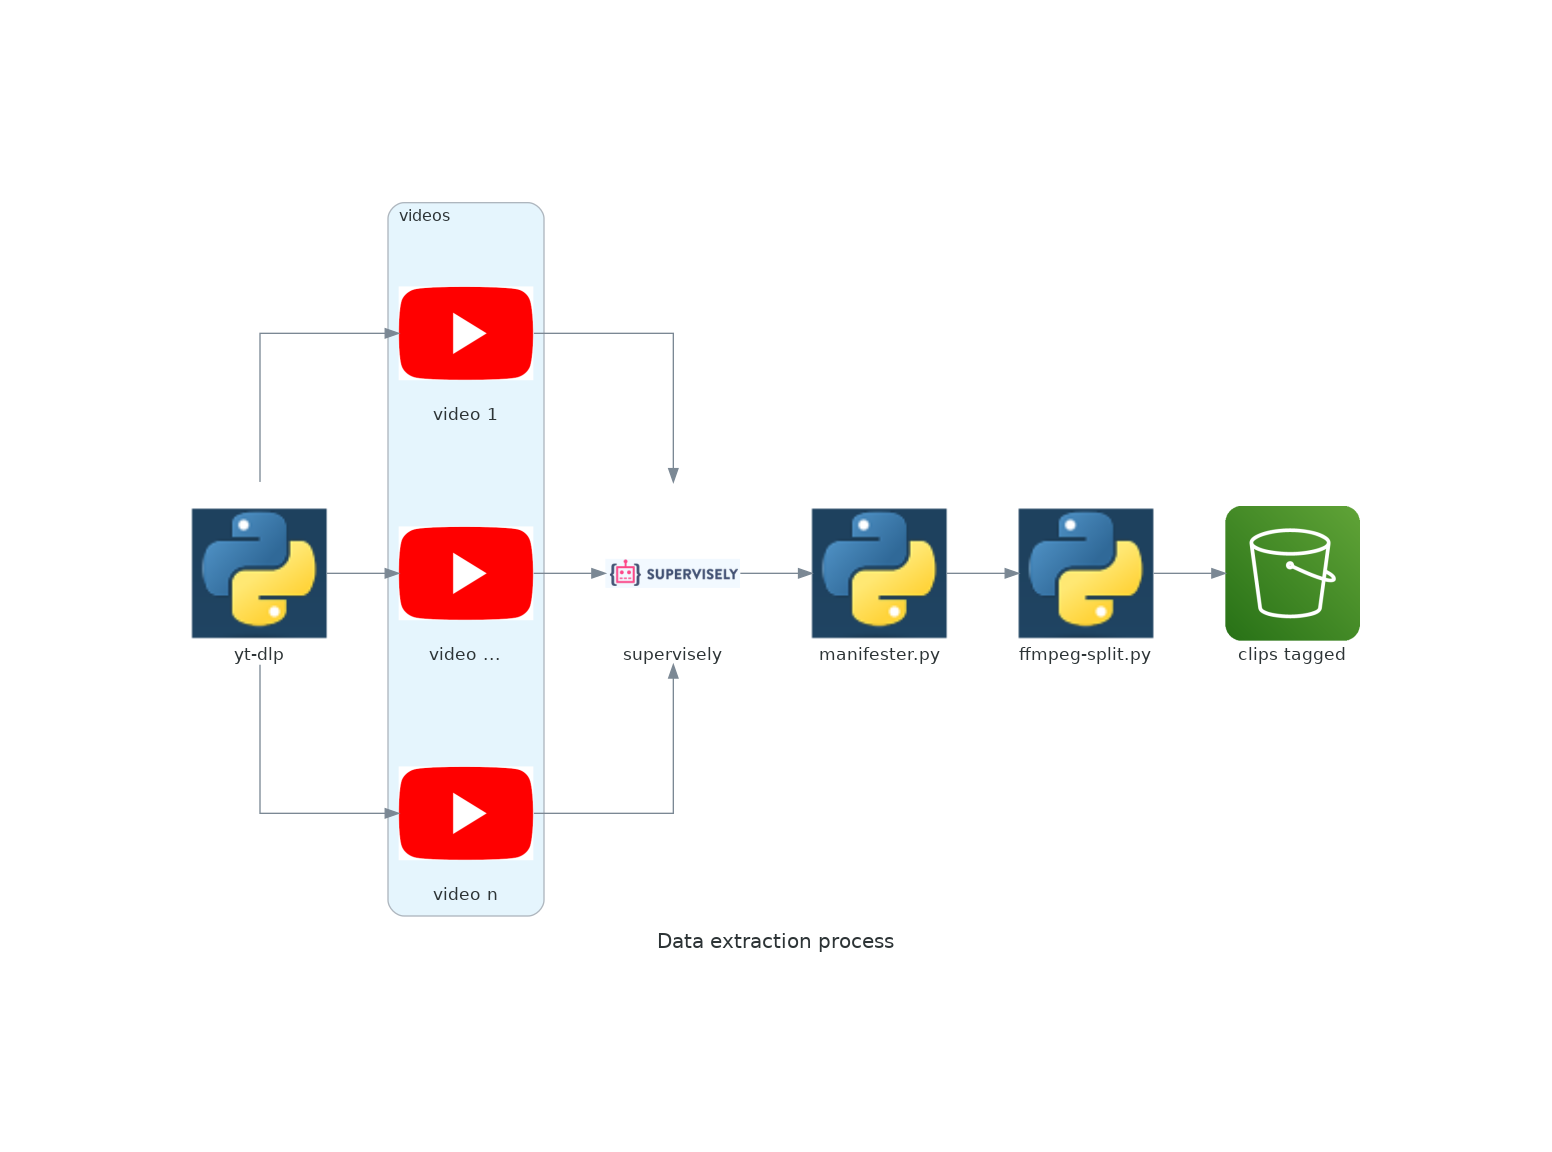
\includegraphics[height=12cm, width=18cm]{figs/data_extraction_process.png}
\end{figure}


\section{Primera sección}
\lipsum[1-5]
\section{Segunda sección}
\lipsum[1-5]
\subsection{Subsección}
\lipsum[1-6]

